%\documentclass[a4paper,10pt]{article}
\documentclass[10pt, conference, letterpaper]{IEEEtran}
\usepackage[utf8]{inputenc}
\usepackage{xspace}
\usepackage{url}
\usepackage{graphicx,graphics} 
\usepackage{color}
\usepackage{amsmath}
\usepackage{amsfonts}
\usepackage{amssymb}
\usepackage{amsthm}
\usepackage{algorithm}
\usepackage{algorithmic}
\usepackage{longtable}
\usepackage{complexity}
\usepackage{tkz-graph}
\usepackage{float}
\usepackage{authblk}
\usepackage{tabularx}
\usepackage{setspace}
\usepackage{icomma}
\usepackage{tkz-graph}
\usepackage{complexity}
\renewcommand{\algorithmicrequire}{\textbf{Input:}}
\renewcommand{\algorithmicensure}{\textbf{Output:}}
\usepackage[colorlinks=true,breaklinks=true,linkcolor=blue]{hyperref}


\newtheorem{proposition}{Proposition}
\newtheorem{theorem}{Theorem}

\setlength{\parskip}{1ex} % Espace entre les paragraphes

\newtheorem{fact}{Fact}
\newtheorem{lemma}[theorem]{Lemma}
\newtheorem{definition}{Definition}
\newtheorem{corollary}{Corollary}

% \renewcommand{\thefootnote}{\*}

\newcommand\pma{\textsc{pma}\xspace}
\newcommand{\todo}[1]{{\color{red} TODO: {#1}}}


\author[1,2]{Ma\"el Guiraud}
\author[1]{Yann Strozecki}
\affil[1]{David Laboratory, UVSQ}
\affil[2]{Nokia Bell Labs France}

%\author{Ma\''el Guiraud\addressmark{1,2}
  %\and Yann Strozecki\addressmark{1}}

%\address{\addressmark{1}David Laboratory, UVSQ, 45 Avenue des Etats Unis, Versailles France \\
  %\addressmark{2}Nokia Bell Labs France, Route de Villejust, Nozay, France}


\title{Scheduling periodic messages on a shared link}

%\keywords{Scheduling}

\begin{document}

\maketitle

%En français
%Ordonnancement de messages périodiques et de leurs réponses sur un lien partagé

%Le Cloud-RAN est une nouvelle architecture de réseau mobile dans laquelle les unités de calcul, traditionnellement 
% installées au pieds des antennes, sont déportées dans des data-centers distants. Dans ces conditions, pour respecter des contraintes liées aux protocoles 4G et 5G, il faut minimiser la latence des messages périodiques envoyés par les antennes
%à leurs unités de calcul. Nous essayons donc ici de trouver des plans périodiques de transmission des messages qui ne nécessitent pas de buffer et donc de latence supplémentaire.

%Dans cet article nous étudions une topologie en étoile, ou la contention vient d'un lien partagé entre toutes les antennes.
%Pour des messages arbitrairement grand, nous montrons qu'il existe toujours un plan de transmission des messages si la charge du réseau est inférieure à $40\%. De plus, nous montrons comment réduire le problème à des messages de taille unitaire
%pour une latence additionnelle modeste.

%Pour les messages de taille $1$, nous donnons un algorithme en temps polynomial qui trouve un plan de transmission
%pour des charges jusqu'à $58\%$. De plus, en analysant un algorithme aléatoire glouton, pour n'importe quelle charge, 
% presque toutes les instances avec suffisamment de messages ont une solution, ce qui explique pourquoi les algorithmes
%gloutons présentés dans l'article marchent si bien en pratique.


%keywords :C-RAN; latency; periodic scheduling; greedy algorithms


\begin{abstract}
Cloud-RAN is a recent architecture for mobile networks where the processing units are located in distant data-centers while, until now, they were attached to antennas. The main challenge, to fulfill protocol time constraints, is to guarantee a low latency for the periodic messages sent from each antenna to its processing unit and back. The problem we address is to find a sending scheme of these periodic messages without contention nor buffering.

We focus on a simple but common star shaped topology, where all contentions are on a single link shared by all antennas. For messages of arbitrary size, we show that there is always a solution as soon as the load of the network is less than $40\%$. Moreover, we explain how we can restrict our study to message of size $1$ without increasing too much the global latency. 

For message of size $1$, we prove that it is always possible to schedule them, when the load is less than $61\%$  using a polynomial time algorithm. Moreover, using a simple random greedy algorithm, we show that almost all instances of a given load admit a solution, explaining why most greedy algorithms work so well in practice.  
\end{abstract}

\section{Introduction}

Next generations of mobile network architectures evolve toward centralized radio network architectures called C-RAN for Cloud Radio Access Network, to reduce energy consumption costs~\cite{mobile2011c} and more generally the total cost of ownership. The main challenge for this type of architecture is to reach a latency compatible with transport protocols~\cite{ieeep802}. The latency is measured between the sending of a message by a Remote Radio Head (RRH) and the receptions of the answer, computed by real-time virtualized network functions of a BaseBand Unit (BBU) in the cloud. For example, LTE standards require to process functions like HARQ (Hybrid Automatic Repeat reQuest) in $3$ms~\cite{bouguen2012lte}. In 5G, some services need end-to-end latency as low as $1$ms~\cite{3gpp5g,boccardi2014five}. The specificity of the C-RAN context is not only the latency constraint, but also the periodicity of the data transfer in the frontaul network between RRHs and BBUs: messages need to be emitted and received each millisecond~\cite{bouguen2012lte}. Our aim is to operate a C-RAN on a low-cost shared switched network. 

 Statistical multiplexing even with a large bandwidth does not satisfies the latency requirements of C-RAN~\cite{dominique2018deterministic,barth2018deterministic}. The current solution~\cite{pizzinat2015things,tayq2017real} is to use dedicated circuits for the fronthaul. Each end-point, an RRH on one side and a BBU on the other side is connected through direct fiber or full optical switches. This eliminates all contentions since each message flow has its own link, but it is extremely expensive and do not scale in the case of a mobile network composed of about $10,000$ base stations. 

The question we address is the following: \emph{is it possible to schedule periodic messages on a shared link without using buffers}? Eliminating this source of latency leaves us with more time budget for latency due to the physical length of the routes in the network, and thus allows for wider deployment areas. Our proposed solution is to compute beforehand a \emph{periodic and deterministic} sending scheme, which completely avoids contention. This kind of deterministic approach has gained some traction recently: Deterministic Networking is under standardization in IEEE 802.1 TSN group~\cite{finn-detnet-architecture-08}, as well at IETF DetNet working group~\cite{ieee802}. Several patents on concepts and mechanisms for DetNet have been already published, see for example~\cite{howe2005time,leclerc2016transmission}. 


The algorithmic problem studied in the present article, called Periodic Message Assignment or \pma, is the following.
Given a period, a message size and delay between the two contention points different for each message, choose an offset (departure time in the period) for each message, so that it goes through the two contention points when they are free. It is  similar to the two flow shop scheduling problem~\cite{yu2004minimizing} with periodicity. The periodicity adds more constraints, since messages from consecutive periods can interact. The objective is usually to minimize the makespan, or schedule length, but in our periodic variant it is infinite. Hence, we choose to look for any periodic schedule without buffering, which minimizes the trip time of each message. 


 To our knowledge, all studied periodic scheduling problems are quite different from the one we present.
Either the aim is to minimize the number of processors on which the periodic tasks are scheduled~\cite{korst1991periodic,hanen1993cyclic}, while our problem corresponds to a single processor and a constraint similar to makespan minimization. In cyclic scheduling~\cite{levner2010complexity}, the aim is to minimize the period of a scheduling to maximize the throughput, while our period is fixed. The train timetabling problem~\cite{lusby2011railway} and in particular the periodic event scheduling problem~\cite{serafini1989mathematical} are generalizations of our problem, since they take into account 
a fixed period and can express the fact that two trains (like two messages) should not cross. However, they are much more general: the trains can vary in size, speed, the network can be more complex than a single track and there are precedence constraints. Hence, the numerous variants of train scheduling problems are very hard to solve (and always $\NP$-hard), they usually allow for some delay and most of the work is devising good algorithms using branch and bound, mixed integer programming, genetic algorithms \dots~\cite{lusby2011railway}


In previous articles of the authors, generalizations of \pma allowing buffers are studied on a single link~\cite{dominique2018deterministic} or on a cycle~\cite{Guir1905:Deterministic}. Heuristics (using scheduling algorithms) and FPT algorithms are used to find a sending scheme with \emph{minimal latency}, while here we only look for sending scheme without any additional latency. More complex problems of computing schedules for time sensitive networks has been practically solved, using mixed integer programming~\cite{nayak2017incremental,steiner2018traffic} or an SMT solver~\cite{dos2019tsnsched}, but without theoretical guarantes on the quality of the produced solutions. Typical applications cited in these works (out of C-RAN) are sensor networks communicating periodically inside a car or a plane, or logistic problems in production lines.



\paragraph{Organization of the paper}

In Sec.~\ref{sec:model}, we present the model and the problem \pma. In Sec.~\ref{sec:large},
we present several greedy algorithms and prove that they always find a solution to \pma for increasing load. Then, we illustrate their surprisingly good performances on random inputs in Sec.~\ref{sec:perf_large}. It turns out that the message size can be assumed to be one for a small price in added latency, as explained in Sec.~\ref{sec:reduction}. Hence, we develop a deterministic and a probabilistic algorithm for this special case in Sec.~\ref{sec:small}, which work for much higher loads than the algorithms for large message size and we illustrate their performances on random inputs in Sec.~\ref{sec:perf_small}.


\section{Model}\label{sec:model}


In this article, we model a simple network (see fig.~\ref{fig:model}) in which periodic messages flow through a single link. The answer to each message is then sent back through the same bidirectional link. The model and problem can easily be generalized to any network, that is any directed acyclic graph with any number of contention points, see \cite{dominique2018deterministic}. We choose here to present the simplest non trivial such network, for which we can still obtain some theoretical results. 

The time is discretized and the process we consider is periodic of fixed integer period $P$. We use the notation $[P]$ for the set $\{0,\dots,P-1\}$. In the C-RAN network we model, represented in Fig.\ref{fig:model}, all messages are of the same nature, hence they are all of the same size denoted by $\tau$. This size corresponds to the time needed to send a message through some contention point of the network, here a link shared by all antennas. We denote by $n$ the number of messages, which are numbered from $0$ to $n-1$. A message $i$ is characterized by its delay $d_i$. It means that if the message number $i$ arrives at the link at time $t$, then it returns to the other end of the link on its way back at time $t + d_i$. 
\begin{center}
\begin{figure}
%\begin{minipage}[c]{.5\linewidth}
\centering
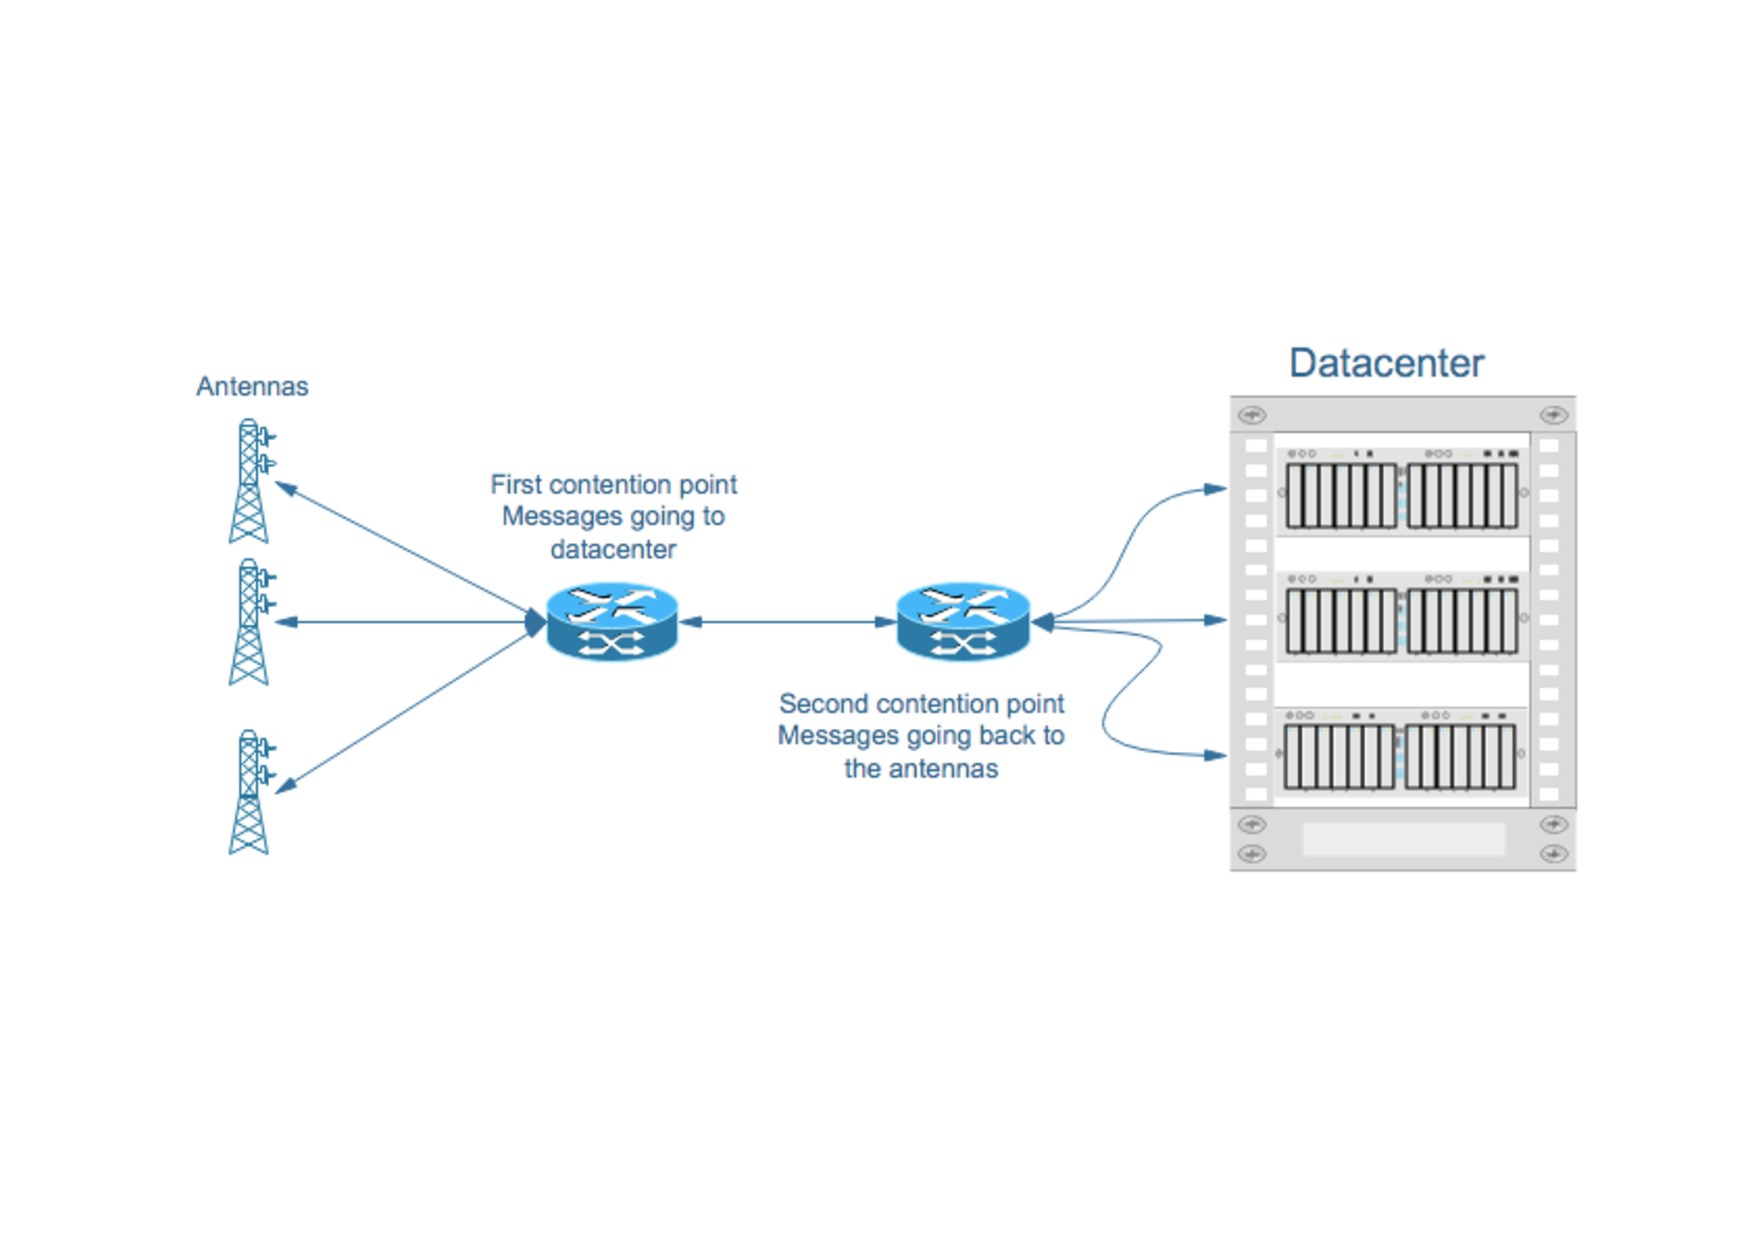
\includegraphics[scale=0.35]{network.pdf}
%\end{minipage}
%\begin{minipage}[c]{.5\linewidth}
\centering
\scalebox{0.5}{
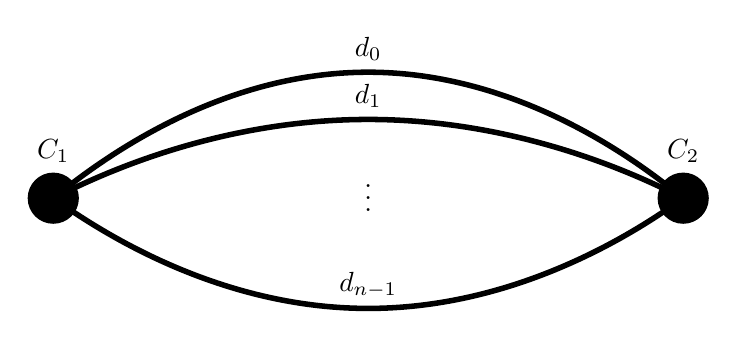
\begin{tikzpicture}
    \SetGraphUnit{5}
      \node[black] at (8,5.9) {$d_0$};
       \node[black] at (4,4.6) {$C_1$};
        \node[black] at (12,4.6) {$C_2$};
         \node[black] at (8,5.3) {$d_1$};
            \node[black] at (8,2.9) {$d_{n-1}$};
            \node[black] at (8,4.15) {.};
            \node[black] at (8,4.0) {.};
            \node[black] at (8,3.85) {.};
  \tikzstyle{VertexStyle}=[shape = circle, draw, minimum size = 10pt]
  \SetUpVertex[FillColor=black]  
  \Vertex[x=4,y=4]{1}
  \Vertex[x=12,y=4]{2}  



  \draw[->,line width=2pt,black] (4,4) parabola bend (8,5.6) (12,4);
  \draw[->,line width=2pt,black] (4,4) parabola bend (8,5) (12,4);
      \draw[->,line width=2pt,black] (4,4) parabola bend (8,2.6) (12,4);

\end{tikzpicture}
}
%\end{minipage}
\caption{An example of a network with two contention points}
\label{fig:model}
\end{figure}
\end{center}

Since the process we describe is periodic, we may consider any interval of $P$ units of time
to represent the state of our system. Describing the messages going through the two contention points during such an interval
completely defines the periodic process. We call the representation of the interval
of time in the first contention point the \emph{first period} and the \emph{second period}
for the second contention point.

An \emph{offset} of a message is a choice of time at which it arrives
at the first contention point. Let us consider a message $i$
of offset $o_i$, it uses the interval of time $[i]_1 = \{ (o_i + t) \mod P \mid 0 \leq t < \tau \}$ in the first period and $[i]_2 = \{ (d_i + o_i + t) \mod P \mid 0 \leq t < \tau \}$ in the second period. We say that two messages $i$ and $j$ collide if either $[i]_1 \cap [j]_1 \neq \emptyset $ or $[i]_2 \cap [j]_2 \neq \emptyset $. If $t \in [i]_1$ (resp. $t \in [i]_2$) we say that message $i$ uses time $t$ in the first period (resp. in the second period).

We want to send all messages, so that they are no collision in the shared link.
In other word, we look for a way to send the messages without using buffering and 
hence limiting the latency to the physical length of the links. An assignment is a
choice of an offset for each message such that \emph{no pair of message collide}, as shown in Fig.~\ref{fig:assignment}.
Formally, an \emph{assignment} is a function from the messages in $[n]$ to their offsets in $[P]$.  

We call Periodic Message Assignment or \pma the problem studied in this article,
which asks, given an instance of $n$ messages, a period $P$ and a size $\tau$, to find 
an assignment or to decide there is none.
\begin{figure}
\begin{center}
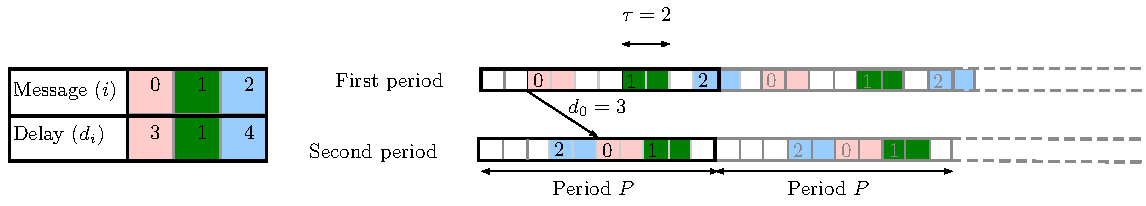
\includegraphics[scale=0.7]{instance}
\end{center}
\caption{An instance of \pma ($3$ messages, $P= 10$ and $\tau = 2$) and one of its assignments}
\label{fig:assignment}
\end{figure}

The complexity of \pma is not yet known. However, we have proven that, when parameterized by
$n$ the number of messages, the problem is \FPT~\cite{barth2018deterministic}.
A slight generalization of \pma, with several contention points but each message only going through two of them, as in \pma, is \NP-hard~\cite{barth2018deterministic}. If the shared link is not bidirectional, that is there is a single contention point and each message goes through it twice, it is also \NP-hard~\cite{orman1997complexity}. Hence, we conjecture that \pma is \NP-hard.

To overcome the supposed hardness of \pma, we study it when the load of the system is small enough. The \emph{load} is defined as the number of units of time used in a period by all messages divided by the period. Hence the load is equal to $n\tau /P$. Our aim is to prove that, for small load, there is \emph{always} an assignment and that it can be found by a polynomial time algorithm.



\section{Greedy Algorithms for Large Messages} \label{sec:large}

In this section, we study the case of large messages. When modeling real problems,
it is relevant to have $\tau > 1$ when the transmission time of a single message is large with regard to its delay.

A partial assignment $A$ is a function defined from a subset $S$ of $[n]$ to $[P]$.
We say that $|S|$, the cardinal of the domain of $A$, is its \emph{size}.
We say that a message in $S$ is \emph{scheduled} (by $A$), and a message not in $S$ is \emph{unscheduled}. We only consider partial assignments such that no pair of messages of $S$ collide. If $A$ has domain $S$, and $i \notin S$, we define the extension of $A$ to the message $i$ by the offset $o$, denoted by $A[i \rightarrow o]$, the function defined as $A$ on $S$ and $A[i \rightarrow o](i) = o$.

All presented algorithms build an assignment incrementally, by growing the size of the domain of a partial assignment. Moreover, the algorithm of this section are greedy since once an offset is chosen for a message, it is never changed.


\subsection{First Fit}


Assume that for some partial assignment $A$, the message $i$ has offset $o$: it uses all times from $o$ to $o + \tau -1$ in the first period. If a message $j$ is scheduled with some offset $o'$ before $o$, then the last time it uses in the first period is $o'+\tau-1$ and it should be less than $o$, which implies that $o' \leq o - \tau + 1$. If $o'$ is larger than $o$, to avoid collision between messages $j$ and $i$, it should be larger or equal to $o+ \tau$. Hence the message $i$ forbids $2\tau -1$ offsets for messages still not scheduled because of this use of time in the first period. The same reasoning can be done for the second period, which again forbids $2\tau -1$ offsets. Hence, if $|S|$ messages are already scheduled, then $|S|(4\tau -2)$ offsets are forbidden for each unscheduled message. Note that this is an upper bound on the number of forbidden offsets, since the same offset can be forbidden twice because of a message on the first and on the second period.


Let $Fo(A)$ be the maximum number of forbidden offsets when extending $A$. Formally, assume $A$ is defined over $S$ and $i\notin S$, $Fo(A)$ is the maximum over all values of $d_i$ of $|\left\{ o \in [P] \mid A[i \rightarrow o] \text{ has no collision }\right\}|$. The previous paragraph shows that $Fo(A)$ is always bounded by $(4 \tau -2)|S|$. 

The first algorithm deals with the route in the order they are given:  for each unscheduled route it tests all offsets from $0$ to $P-1$ until one do not create a collision with the current assignment.
We call this algorithm \emph{First Fit}. Remark that if $Fo(A) < P$, then whatever the delay of the route we want to extend $A$ with, it is possible to find an offset. Since $Fo(A) \leq (4 \tau -2)|S|$ and $|S| < n$, First Fit (or any greedy algorithm) will always succeed when $(4 \tau -2)n \leq P$, that is when the load $ n\tau /P$ is less than $1/4$.
It turns out that First Fit always creates compact assignments (as defined in~\cite{dominique2018deterministic}), that is a message is always next to another one in one of the two period. Hence, we can prove a better bound on $Fo(A)$, when $A$ is built by First Fit, as stated in the following theorem.

\begin{theorem}
First Fit always solves \pma positively on instances of load less than $1/3$. 
\end{theorem}
\begin{proof}
To prove the theorem, we show by induction on the size of $S$, that $Fo(A) \leq |S|(3\tau -1) + \tau -1$.  For $S = 1$, it is clear since a single message forbid at most $(3\tau -1) + \tau -1 = 4\tau-2$ offsets, as explained before. Now, assume $Fo(A) \leq |S|(3\tau -1) + \tau -1$ and consider a route $i \notin S$ such that First Fit builds $A[i \rightarrow o]$ from $A$. By definition of First Fit, choosing $o-1$ as offset creates a collision. W.l.o.g. say it is a collision in the first period. It means that there is a scheduled message between $o - \tau $ and $o-1$ (modulo $P$), hence all these offsets are forbidden by $A$. The same offsets are also forbidden by the choice of $o$ as offset for $i$, then only $3\tau -1$ new offsets are forbidden, that is $Fo(A[i \rightarrow o]) \leq Fo(A) + (3\tau -1)$, which proves the induction and the theorem.
\end{proof}


\subsection{Meta-Offset}

The second method is described  in~\cite{dominique2018deterministic} and achieves the same bound on the load using a different method, that we recall here because we use it in the more involved algorithm of the next section.
The idea is to restrict the possible offsets at which messages can be scheduled. It seems counter-intuitive, since it decreases artificially the number of possible offsets to schedule new messages. However, it allows to reduce the number of forbidden offsets, when the algorithm is designed accordingly. A \emph{meta-offset} is an offset of value $i\tau$,
with $i$ an integer from $0$ to $P / \tau$. We call Meta-Offset the greedy algorithm
which works as First Fit, but consider only meta-offsets when scheduling new messages. 

Let $Fmo(A)$ be the maximal number of meta-offsets forbidden by $A$. 
 By definition, two messages with a different meta-offset cannot collide in the first period.
Hence, $Fmo(A)$ can be bounded by $3|S|$ and we obtain the following theorem.


\begin{theorem}[Proposition 3 of~\cite{dominique2018deterministic}]
Meta-Offset always solves \pma positively on instances of load less than $1/3$.
\end{theorem}

\subsection{Tuples and meta-intervals}

We now propose a more involved family of greedy algorithms which 
solves \pma positively for larger loads. We try to combine the good properties of the two previous algorithms: the compacity of the assignments produced by First Fit and the use of meta-offsets to reduce collisions on the first period. The idea is to schedule several messages at once, using meta-offsets, to maximize the compacity of the obtained solution. 
We first describe the algorithm which schedules pairs of routes and then explain quickly how we can extend it by scheduling any tuples of messages instead of pairs.

We first prove a lemma which allows to assume that the period $P$ is a multiple of $\tau$, since it makes the analysis of our algorithms much simpler and tighter. It only changes the load from $n \tau / P$ to at most $n (\tau +1)/ P$: the difference is less than $n /P < 1/\tau$, and thus very small for large $\tau$.

\begin{lemma}
Let $I$ be an instance of \pma with $n$ messages of size $\tau$, period $P$ and $m = P / \tau$. There is an instance $I'$ with $n$ messages of size $\tau'$ and period $P'= m\tau'$ such that an assignment of $I'$ can be transformed into an assignment of $I$ in polynomial time.
\end{lemma}
\begin{proof}
Let $P = m \tau + r$ with $r \leq \tau$. We define the instance $I'$ as follows: $P' = mP$, $d_{i}' = m d_i$ and $\tau' = m \tau + r$. With this choice, we have $P' = m(m \tau + r) = m \tau'$.
Consider an assignment $A'$ of the instance $I'$.
If we let $\tau'' = m\tau$, then $A'$ is also an assignment for $I'' = (P',\tau'',(d_{0}',\dots,d_{n-1}'))$. Indeed, the size of each message, thus the intervals of time used in the first and second period begin at the same position but are shorter, which cannot create collisions.
We then use a compactification procedure as in~\cite{barth2018deterministic}. The first message is positioned at offset zero. The first time it uses in the second period is a multiple of $m$ since its delay is by definition a multiple of $m$. Then, all other messages are translated to the left by removing increasing integers to their offsets, until there is a collision. It guarantees that some message is in contact with the first one on the first or second period,  which implies that its offset is a multiple of $m$. This procedure can be repeated until we get some solution $A''$ to $I''$, such that all positions of messages in the first and second period are multiples of $m$. Hence, if we define $A$ as $A(i) = A''(i)/m$, we obtain an assignment of $I$.
\end{proof}

From now on, we always assume that $P = m\tau$ and the load is then $n/m$.
We are interested in the remainder modulo $\tau$ of the delays of each message.
We write $d_i = d_{i}'\tau + r_i$ and assume from now on that messages are sorted by increasing $r_i$.
A \emph{compact pair}, as shown in Fig.~\ref{fig:compactpair} is a pair of messages $(i,j)$ with $i < j$ such that we can put them next to each other in the second period using meta-offsets.
We have $r_i \leq r_j$ since $i < j$. We denote by $g$ the gap between the two messages in the first period, that we define by $d_{i}' = g + 1 + d_{j}' \mod m$. We require that $g \neq 0$ so that there are no collision in the first period if we schedule these two messages such that the difference of their offsets is the gap. 

\begin{figure}[h]
\begin{center}

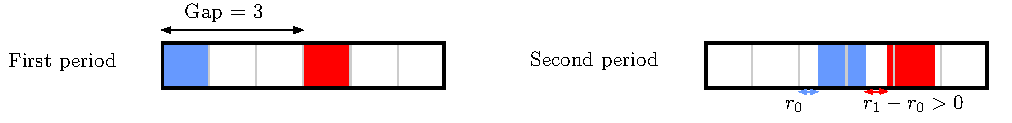
\includegraphics[scale=0.7]{compact_pair}
\end{center}
\caption{Representation of a compact pair scheduled using meta-offsets}
\label{fig:compactpair}
\end{figure}

\begin{lemma}\label{lemma:pair_find}
Given $3$ messages, two of them always form a compact pair. 
\end{lemma}
\begin{proof}
If the first two messages or the first and the third message form a compact pair,
then we are done. If not, then by definition $d_{1}' = 1 + d_{2}' = 1 + d_{3}'$. Hence, the messages $2$ and $3$ have the same delay and form a compact pair of gap $1$.
\end{proof}

We call \emph{Compact Pairs} the following greedy algorithm. From the $n$ routes in order
of increasing $r_i$, we build a sequence of at least $n/3$ compact pairs using Lemma~\ref{lemma:pair_find}. They are then scheduled in the order they have been built using meta-offsets only. If at some point all compact pairs are scheduled or the current one cannot be scheduled, the remaining messages are scheduled as in Meta-Offset. The analysis of the algorithm relies on the evaluation of the number of forbidden meta-offsets. In the first phase of the algorithm, one should evaluate the number of forbidden offsets when scheduling a compact pair, that we denote by $Fmo_2(A)$. In the second phase, we need to evaluate $Fmo(A)$. When scheduling a message in the second phase, a scheduled compact pair only forbids \emph{three} meta-offsets in the second period. If messages in a pair are scheduled independently, they forbid \emph{four} meta-offsets, which explains the improvement from Meta Offset. We first give a simple lemma, whose proof can be read from Fig.~\ref{fig:forbidenmeta}, which allows to bound $Fmo_2(A)$ and to lower bound the number of scheduled compact pairs.

\begin{lemma}\label{lemma:pair_forbid}
A compact pair already scheduled by Compact Pair forbids at most four meta offsets in the second period to another compact pair when it is scheduled by Compact Pair.
\end{lemma}

\begin{figure}
\begin{center}
\includegraphics[scale=0.7]{pairforbiden}
\end{center}

\caption{Representation of the meta offsets forbidden by a compact pair in blue when scheduling a compact pair in red} 
\label{fig:forbidenmeta}
\end{figure}
\begin{theorem}
Compact Pairs always solves \pma positively on instances of load less than
$3/8$.
\end{theorem}
\begin{proof}
Let $n_2$ be the number of compact pairs scheduled in the first phase. When scheduling a new pair, the position of the $2n_2$ messages on the first period forbid $4n_2$ offsets for a compact pair. Indeed, each scheduled message can collide
with each of the two messages which form a compact pair. On the second period, we can use Lemma~\ref{lemma:pair_forbid} to bound the number of forbidden offsets by $4n_2$. 
Hence, we have established that during the first phase, the partial solution $A$
satisfies $Fmo_2(A) \leq 8n_2$. This first phase continues while there is possible offsets for compact pairs, which is the case when $Fmo_2(A) \leq m$, that is while $n_2 \leq m/8$.
In the second phase, a compact pair forbids $3$ meta offsets in the 
second period and $2$ in the first. Hence, if we let $n_1$ be the number of messages scheduled in the second phase to give the assignment $A$, we have $Fmo(A) \leq n_2*5 + n_1*3$. 
The algorithm can always schedule messages when $Fmo(A)$ is less than $m$, thus
$$ n_2*5 + n_1*3 \leq m$$
$$ n_1 \leq \frac{8m - 5m }{24}$$
$$n_1 \leq \frac{m}{8}$$

Hence, we can guarantee $n_1 = \frac{m}{8}$ and the number of routes scheduled is at least $2n_2 + n_1$,
which is $\frac{3}{8}m$. Remark that we need to be able to schedule two third of the messages as compact pairs, which is possible by Lemma~\ref{lemma:pair_find}. Therefore an assignment is always produced when the load is less then $\frac{3}{8}$.
\end{proof}

The algorithm can be improved by forming compact tuples instead of compact pairs.
A compact $k$-tuple is a sequence of messages $i_1 < \dots < i_k$ (with $r_{i_1},\dots,r_{i_k}$ increasing), for which meta-offsets can be chosen so that there is no collision,
the messages in the second period are in order $i_1,\dots,i_k$ and two consecutive messages $i_{l},i_{l+1}$ use the times $o$ and $o + r_{i_{l+1}} -r_{i_{l}} + \tau$ in the second period.

The algorithms \emph{Compact k-tuples} works by scheduling compact $k$-uples
using meta offsets while possible, then scheduling compact $k-1$-uples and so on until $k=1$.
The theorem we give is obtained for $k=10$, but taking arbitrary large $k$ and using more refined bounds on $Fmo(A)$ is not enough to prove the same theorem for a load of $41/100$ and only works for larger $n$.


\begin{lemma}\label{lemma:uple_find}
Given $k^3/3 + 1$ messages, $k$ of them always form a compact $k$-tuple. 
\end{lemma}
\begin{proof}
We prove the property by induction on $k$. We have already proved it for $k=2$ in Lemma~\ref{lemma:pair_find}.
Now assume that we have found $C$ a compact $(k-1)$-tuple in the first $(k-1)^3/3$
messages. Consider the next $k(k-1)$ messages. If $k$ of them have the same delay,
then they form a compact $k$-tuple and we are done. Otherwise, there are at least $k$ different values
in those $k(k-1)$ messages. By the pigeonhole principle, one of this delay allows to extend $C$, since 
a compact $(k-1)$-tuple forbid $k-1$ values of delay. Since $(k-1)^3/3 + k(k-1) \leq k^3/3$ it proves the induction and the lemma.
\end{proof}


\begin{theorem}
Compact $10$-tuples always solves \pma positively on instances of load less than $4/10$, for instances with $n$ large enough.
\end{theorem}
\begin{proof}
Lemma~\ref{lemma:uple_find} ensures there are compact $k$-tuples, if there are enough messages,
thus $n$ should be larger than $k^3/3 +1$. 
We need the following fact, which generalizes ~\ref{lemma:pair_forbid}. A $k$-tuples forbids $k+j+1$ offsets in the second period when scheduling a $j$-tuple. If the remainder of the messages in the $j$-tuples are larger than the remainder in the $k$-tuples, it forbids $k+j$ messages only.
It allows to compute a lower bound on the number of scheduled $i$-tuples for $i$ equal $k$ down to $1$ by bounding $Fmo_i(A)$, the number of forbidden meta-offsets when placing $i$-tuple in the algorithm.
If we denote by $n_i$ the number of compact $i$-tuples scheduled by the algorithm,
we have the following equation:  $$ Fmo_i(A) \leq \displaystyle{\sum_{j=i}^k n_j(j*i + j + i+ 1)}.$$
The equation for $n_1$ is slightly better: 
$$ Fmo(A) \leq \displaystyle{\sum_{j=1}^k n_j(2j + 1)}.$$
A bound on $n_i$ can be computed, since $A$ can be extended while $Fmo_i(A) < m$. A numerical computation of the $n_i$'s shows that the algorithm always finds a solution when the load is less than $4/10$.
\end{proof}

The code computing the $n_i$ can be found on the author's website at \url{https://yann-strozecki.github.io/}.
To make the algorithm Compact $10$-tuples work, we need to have enough messages to be able to
produce enough compact $10$-tuples. Theoretically, we need more than $333$ messages. This bound can be improved
by a better algorithm to find compact tuples than the one described in Lemma~\ref{lemma:uple_find}. On random instances, the probability that $k$ messages do not form a compact $k$-tuples is low, and we can just build the tuples greedily. Therefore, for random instances, forming compact $k$-uples is almost never a problem and the algorithm works even for small $n$.

\subsection{Experimental Results} \label{sec:perf_large}

We present results of simulations of the algorithms presented above, to experimentally assess their performance on
random instances. The implementation in C of these algorithms can be found on the author's website at \url{https://yann-strozecki.github.io/}. We experiment with several periods and message sizes. For each set of parameters, we try every possible load by changing the number of messages and give the success rate of each algorithm. The success rate is measured on $10000$ instances of \pma generated by drawing uniformly and independently the delays of each message in $[P]$. 

The algorithms we consider are the following:
\begin{itemize}
	\item First Fit
	\item Meta Offset
	\item Compact Pair
	\item Greedy Uniform (see Sec.~\ref{sec:small})
	\item Exact Resolution using an algorithm from~\cite{dominique2018deterministic}  
\end{itemize}

On a regular laptop, all algorithms terminates in less than a second when solving $10000$ instances with $100$ messages except the exact resolution, whose complexity is exponential in the number of routes (but polynomial in the rest of the parameters). Hence, the theoretical best value given by the exact resolution is only available in the experiment with at most $10$ messages. 
\begin{figure}
\begin{center}
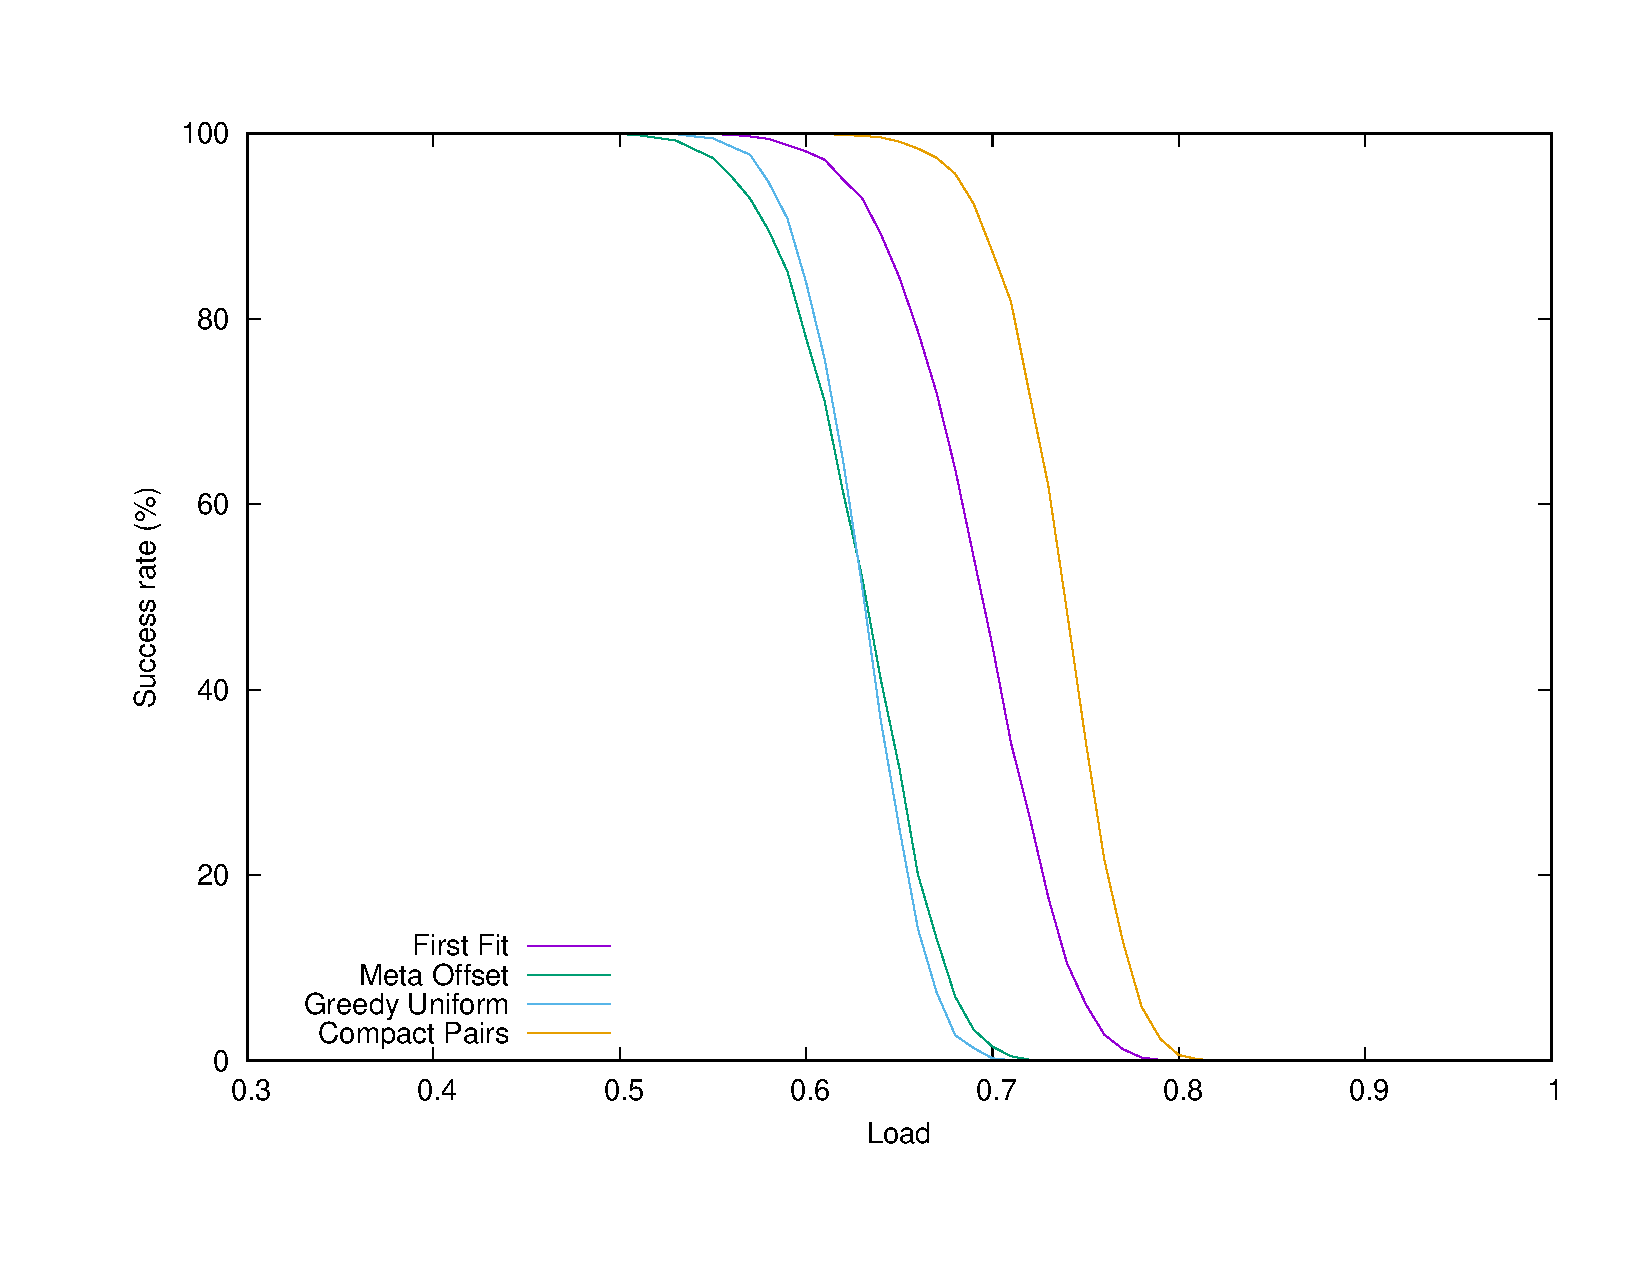
\includegraphics[scale=0.3]{100messBig}
\end{center}
\caption{Experiment for $\tau = 1000$, $P=100,000$}
\label{fig:100messBig}
\end{figure}

\begin{figure}
\begin{center}
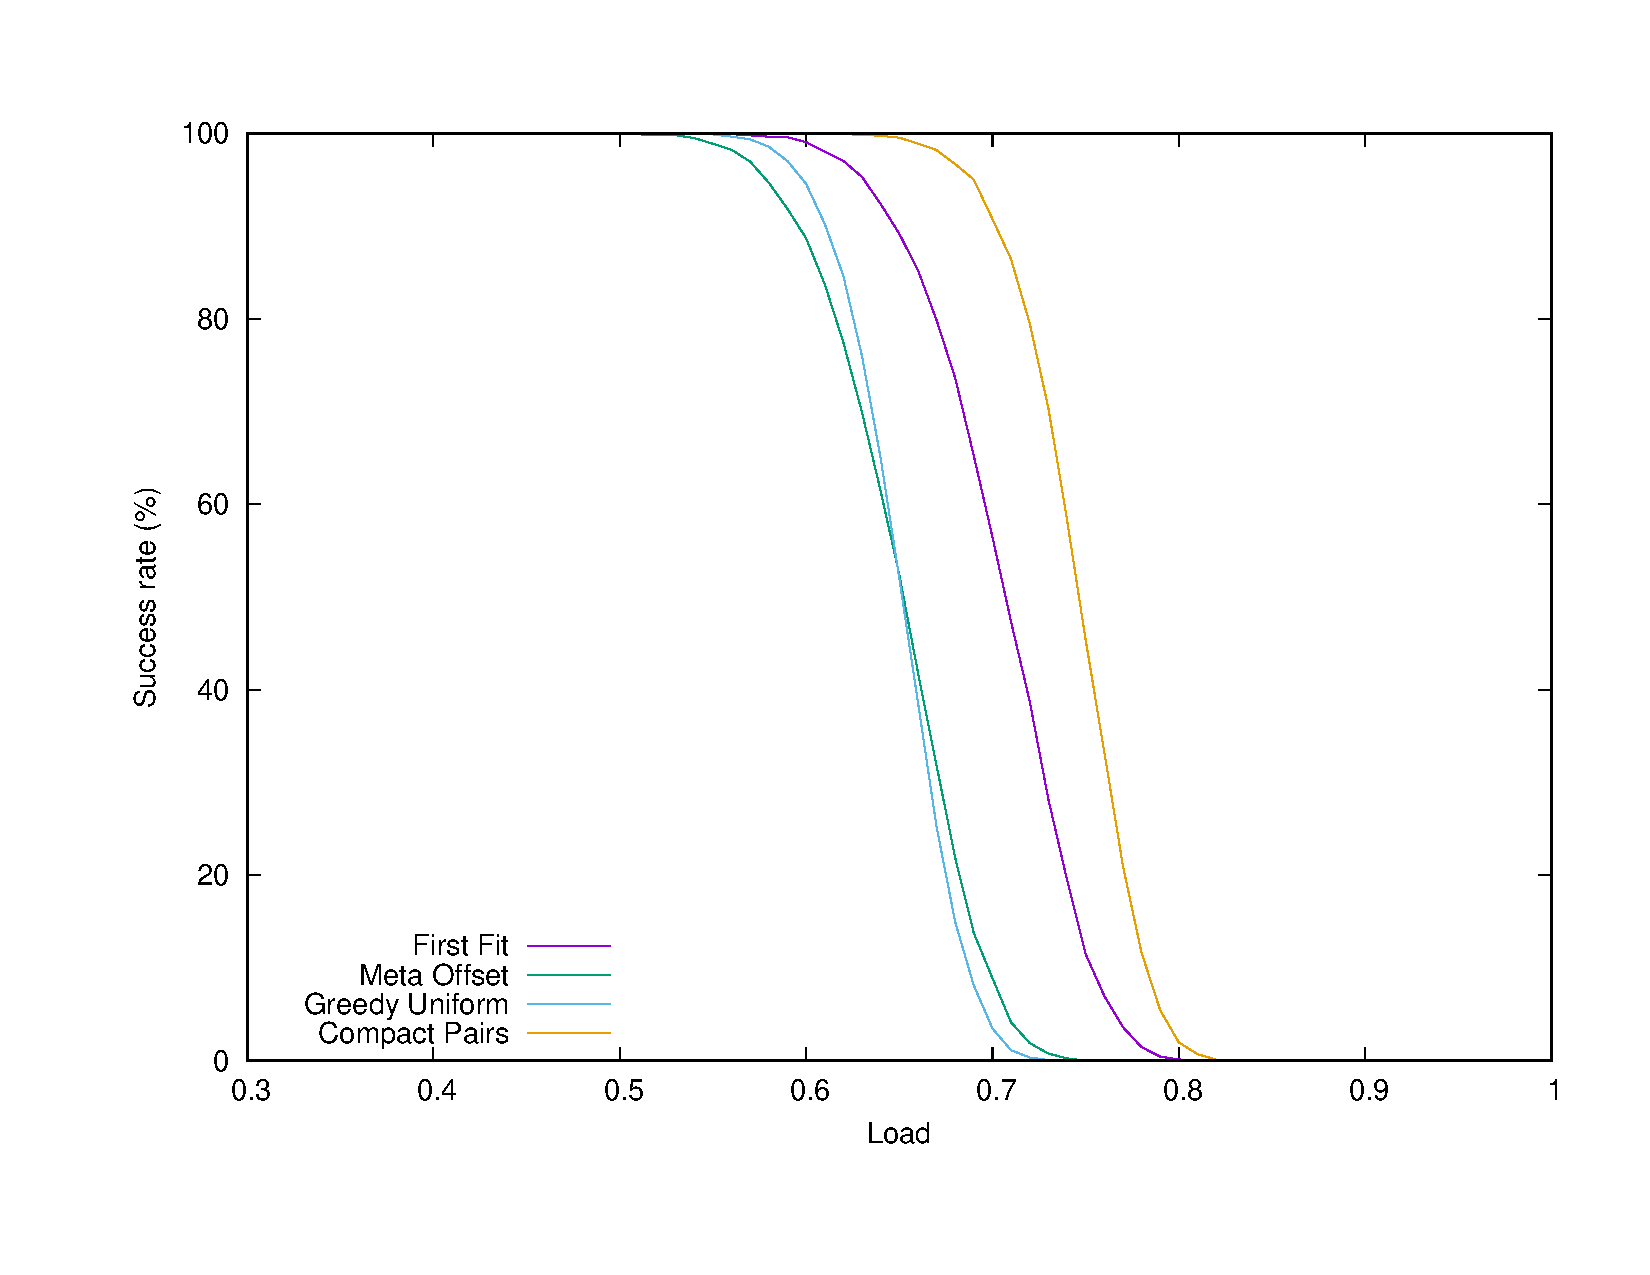
\includegraphics[scale=0.3]{100messSmall}
\end{center}
\caption{Experiment for $\tau = 10$, $P=1,000$}
\label{fig:100messSmall}
\end{figure}

\begin{figure}
\begin{center}
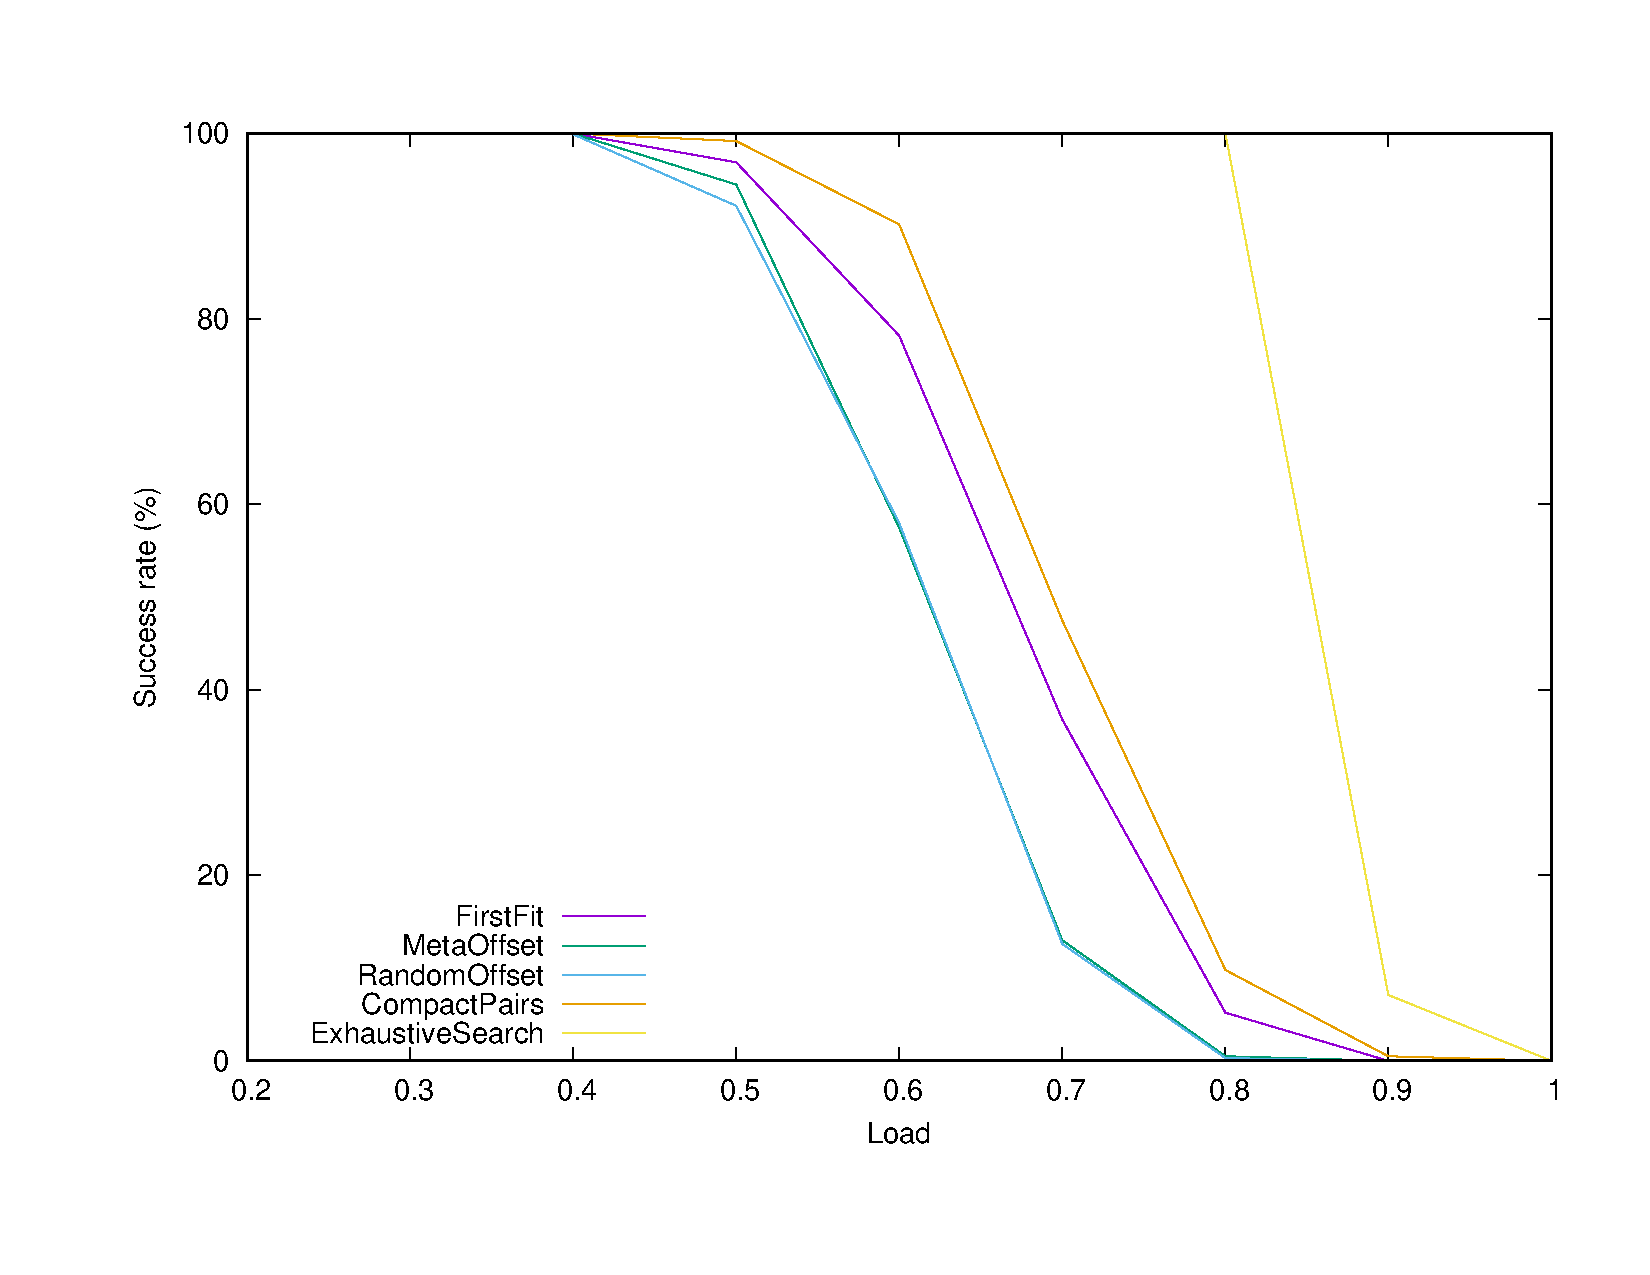
\includegraphics[scale=0.3]{10mess}
\end{center}
\caption{Experiment for $\tau = 1000$, $P=10,000$}
\label{fig:10mess}
\end{figure}

For the tree sets of parameters, the algorithms have the same relative performances. Meta Offset and Greedy Uniform
perform the worst and have almost equal success rate. Remark that they have a $100\%$ success rate for load
less than $1/2$ while it is easy to build an instance of \pma of load $1/3 +\epsilon$ which makes them fail. 
The difference between the worst case analysis and the average case analysis is explained for Greedy Uniform in Sec.~\ref{sec:small}.

First Fit performs better than Meta Offset while they have the same worst case.  Compact Pair, which is the best theoretically also performs the best in the experiments, always finding assignments for load of 
$0.6$. As Shown in Fig.\ref{fig:100messBig} and Fig.\ref{fig:100messSmall}, it appears that the size of the messages have little impact on the success rate of the algorithms. Comparing Fig.\ref{fig:10mess} and Fig.\ref{fig:100messBig} shows that with more messages, the transition between success rate of $1$ to a success rate of $0$ is faster.
Finally, the results of Exact Resolution in Fig.~\ref{fig:10mess} show that the greedy algorithm are fare from always finding 
a solution when it exists. Moreover, we have found an instance with load $0.8$ with no assignment, which gives an upper bound on the highest load for which there is always a solution to \pma.

 

\section{From Large Message to Message of Size one}\label{sec:reduction}

In this section, we explain how we can restrict ourselves to the study of \pma
with small $\tau$ and even $\tau = 1$ if we increase the load or are willing to accept some buffering in our original problem.


\subsection{Reduction without buffering}

We give a reduction from an instance of \pma to another one with the same period and number of messages but 
the size of the messages is doubled. From $I = (P,\tau,(d_{0},\dots,d_{n-1}))$, we build $I' = (P, 2\tau, (d_{0}',\dots,d_{n-1}'))$, where $d_i' = d_{i} - (d_{i} \mod 2\tau)$. The instance $I'$ has a load twice as large as $I$.
On the other hand, all its delays are multiples of $2\tau$ hence solving \pma on $I'$ is equivalent to solving it on $I'' = P/2\tau, 1,d_{0}/ 2\tau,\dots,d_{n-1} /2\tau))$. 

We show that an assignment $A'$ of $I'$ can be transformed into an assignment $A$ of $I$. 
Consider the message $i$ with offset $A'(i)$, it uses all times between $A'(i)$ and $A'(i) + 2\tau -1$ in the first period and all times between $A'(i) + d_{i} - (d_{i} \mod 2\tau)$ to $A'(i) + 2\tau -1+ d_{i} - (d_{i} \mod 2\tau)$. 
If $d_{i} \mod 2\tau < \tau $, we set $A(i) = A'(i)$, and the message $i$ of $I$ is scheduled ``inside'' the 
message $i$ of $I'$, see Fig.~\ref{fig:transf_2tau}. If $\tau \leq d_{i} \mod 2\tau < 2\tau$, then we set 
$A(i) = A'(i) - \tau$. There are no collision in the assignment $A$, since all messages in the second period use
times which are used by the same message in $A'$. In the first period, the messages scheduled by $A$ use either the first
half of the same message in $A'$ or the position $\tau$ before, which is at worst the second half of the times used by another message in $A'$ and thus is not used in $A$.

\begin{figure}[h]
\begin{center}

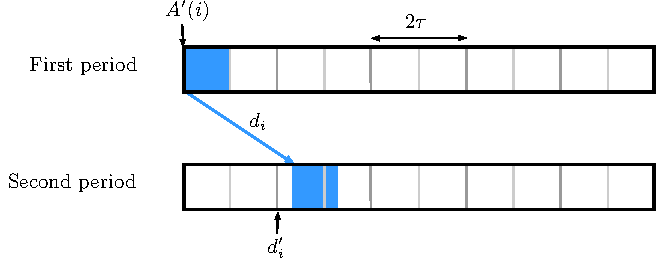
\includegraphics[scale=0.7]{transfo2tau}
\end{center}
\caption{Building $I$ from $I'$}
\label{fig:transf_2tau}
\end{figure}

\subsection{Reduction using buffering}

We have presented our problem with a single degree of freedom by message: its
offset. We could also allow to buffer a message $i$ during a time $b$ between the two contention points, which means changing $d_i$ to $d_i + b$. The quality of the solutions obtained for such a modified instance of \pma are worst since the buffering adds latency to the messages. We now describe how we can make a trade-off between the added latency and the size of the messages, knowing that having smaller messages helps to schedule instances with higher load.


All messages are buffered enough time so that their $d_i$ have the same
remainder modulo $\tau$. It costs at most $\tau$ of buffering, which is not
so good, since algorithms optimizing the latency do better for random instances, see~\cite{barth2018deterministic}. However, it is much better than buffering for a time $P$, the only value for which we are guaranted to find an assignment, whatever the instance. We can choose the message with the longest route as reference remainder, hence this message needs zero buffering. However, the message with the second longest route may have a remainder of $\tau -1$, thus the worst case increase of total latency is $\tau -1$. When all delays are changed so that $d_i$ is a multiple of $\tau$, we have an easy reduction to the case of $\tau = 1$, by dividing all values by $\tau$.

We can do the same kind of transformation by buffering all 
messages, so that $d_i$ is a multiple of $\tau / k$. The cost in term
of latency is then at most $\tau / k$ but the reduction yields messages of size $k$.
For small size of messages, it is easy to get better algorithm for \pma, in particular for $\tau = 1$ as we show in the next section. Here we show how to adapt Compact Pairs to the case of $\tau = 2$.

\begin{theorem}
Compact Pairs on instances with $\tau =2$ always solves \pma positively on instances of load less than $4/9$.
\end{theorem}
\begin{proof}
We assume w.l.o.g that there are less message with even $d_i$ than odd $d_i$.
We schedule compact pairs of messages with even $d_i$, then we schedule single message with odd $d_i$. The worst case is when there is the same number of the two types of messages. In the first phase, if we schedule
 $n/2$ messages, the number of forbidden offsets is $(2 + 3/2)n/2 = 7n/4$. In the second phase,
 if we schedule $n/2$ additional offsets, the number of forbidden offsets is bounded by 
$ (1 + 3/2) n/2  + (1 + 1)n/2 = 9n/4$.
Hence, both conditions are satisfied and we can always schedule messages when $n \leq (4/9)m$.
\end{proof}


We now prove that we can do the previous reduction with $\tau=1$ while optimizing the average added latency. It reduces by a factor of two the average latency. The only degree of freedom in the reduction is the choice of the reference remainder since all other delays are then modified to have the same remainder.
Define the average buffer time for a choice $t$ of reference by $B(t)$. 
If we sum $B(t)$ for $t=0$ to $\tau-1$, the contribution of each message 
will be $\sum_{i=0}^{\tau-1} i$. Since there are $n$ messages, the sum of the $B(t)$ for all $t$ is $n \tau (\tau-1)/2$. There is at least one term of the sum less than the average,
hence there is a $t_0$ such that $B(t_0) \leq n (\tau-1)/2$. In other word, the average
delay for a message, with this choice of reference is less than $(\tau -1)/2$.


\section{Messages of Size One} \label{sec:small}

When $\tau = 1$, \emph{any greedy algorithm} finds a solution to \pma when the load is less than $1/2$ since $Fo(A) \leq (4\tau -2)|S| = 2|S|$ where $S$ is the number of scheduled messages. We now give a method which always finds a solution for load of $1/2 + \epsilon$.

\subsection{Deterministic algorithm}

To go above $1/2$ of load, we use an algorithm which optimizes a potential measuring how many offsets are available for all messages, scheduled or not. Messages are scheduled while possible using any greedy algorithm.
Then, when all unscheduled messages have no free offset, we use a swap operation defined later, which improves the potential. When the potential is high enough, it ensures that there are two messages whose offset can be changed so that a new message can be scheduled. 

 The algorithm is not greedy, since we allow to exchange a scheduled message with an unscheduled one. It cannot work online, since it requires to know all delays of the messages in advance. 

\begin{definition}
The potential of a message of delay $d$, for a partial assignment $A$
is the number of integers $i \in [P]$ such that $i$ is used in the first period and $i+d \mod P$ is used in the second period.
\end{definition}

The potential of a message counts favorable configurations in terms of forbidden offsets.
Indeed, when $i$ is used in the first period and $i+d \mod P$ is used in the second period,
then the same offset is forbidden \emph{twice} for a message of delay $d$. Hence, the potential of a message is related to the number of possible offsets as stated in the following lemma. 

\begin{lemma}
Given a partial assignment $A$ of size $s$, and an unscheduled message of potential 
$v$, there are $P - 2s + v$ possible offsets which can be used to schedule it while extending $A$.
\end{lemma}

For our algorithm, we need a global measure of quality of a partial assignment, 
that we try to increase when the algorithm fail to schedule new messages. 
We call our measure \emph{the potential of an assignment} and we denote it by $Pot(A)$, it is the sum of potentials for $A$ of all messages in the instance.


\begin{definition}
The potential of a position $i$, for a partial assignment $A$, is the number of messages of delay $d$ such that $i+d \mod P$ is used by a route scheduled by $A$. 
\end{definition}

Instead of decomposing the global potential as a sum over the messages, it can be understood
as a sum over positions which gives the next two lemmas.

\begin{lemma}\label{lemma:pot_pos}
The sum of potentials of all positions used in the first period by messages scheduled by $A$ is equal to $Pot(A)$.  
\end{lemma}

By definition of the potential of the positions, we have the following simple invariant.

\begin{lemma}\label{lemma:inv}
The sum of potentials of all positions for a partial assignment with $k$ scheduled messages is $nk$.  
\end{lemma}

 As a consequence of this lemma, $Pot(A) \leq nk$ and in the algorithm we 
 propose, we guarantee to obtain at last half this value by an exchange mechanism, that we call a swap.
Let $A$ be some partial assignment of size $s$ and let $i$ be an unscheduled message of delay $d$. 
Assume that $i$ cannot be used to extend $A$. The swap operation is the following: 
select a free position $o$ in the first period, remove the message which uses the position $o+d$ in the second period from $A$ and extend $A$ by $i$ with offset $o$. We denote this operation by $Swap(i,o,A)$.

\begin{lemma}\label{lemma:swap}
Let $A$ be some partial assignment of size $k$ and let $i$ be an unscheduled message. If $i$ cannot be used to extend $A$, then either $Pot(A) \geq kn/2$ or there is an $o$ such that $Pot(Swap(i,o,A)) > Pot(A)$.
\end{lemma}

\begin{proof}
The positions in the first period can be partitioned into two parts: $P_{u}$ the positions used by some scheduled message and $P_{f}$ the positions unused.
Let $V_f$ be the sum of the potentials of the positions in $P_f$ and by $V_u$ the sum of the potentials of the positions of $P_u$. By Lemma~\ref{lemma:pot_pos}, since $P_f$ and $P_u$ partitions the positions, we have $V_f + V_u = kn$. Moreover, by Lemma~\ref{lemma:pot_pos}, $Pot(A) = V_u$, then $V_f + Pot(A) = kn$.

By hypothesis, since $i$ cannot be scheduled, for all $p \in P_{f}$, $p+d_i$ is used in the second period. We now define the function $F$ which associates to $p \in P_{f}$ the position $A(j)$ such that there is a scheduled route $j$ which uses $p+d$ in the second period, that is $A(j) + d_j = p + d \mod P$. The function $F$ is an injection from $P_{f}$ to $P_u$. Remark now that, if we compare $Swap(i,p,A)$ to $A$, on the second period the positions are used. Hence, the potential of each position stay the same after the swap. As a consequence, doing the operation $Swap(i,p,A)$ add to $Pot(A)$ the potential of the position $p$ and removes the potential of the position $F(p)$. 

Assume now, to prove our lemma, that for all $p$, $Pot(Swap(i,p,A)) \leq Pot(A)$. It implies that for all $p$, the potential of $p$ is smaller than the potential of $F(p)$. Hence, since $F$ is an injection from $P_f$ to $P_u$, we have that $V_f \leq V_u = Pot(A)$. Since $V_f + Pot(A) = kn$, we have that $Pot(A) \geq kn/2$.
\end{proof}

Consider an assignment of size $n' = (1/2 + \epsilon')P$, and a message of delay $d$.
If we consider all $n'$ used offsets $o$ and all times time $o+d$ in the second period, 
then $o$ and $o+d$ are both used for at least $n' - (P -n') = 2\epsilon' P$ values of $o$.
The potential of a message is then larger than $2\epsilon' P$ and when it cannot be scheduled
it is also less or equal to $2\epsilon' P$, that is equal to $2\epsilon' P$.

Hence, the potential of any assignment of size $n'$ is at least $2\epsilon' P n $. As a consequence, the method of Lemma~\ref{lemma:swap} will guarantee a non trivial potential for $2\epsilon' P n <  nn'/2$, that is $\epsilon' < 1/6$. Any algorithm relying on the potential and the Swap operation cannot be guaranteed to work for load larger than $2/3 = 1/2 + 1/6$ or we should either improve on the Swap method or its analysis. In particular, $2\epsilon P$ positions in $P_{u}$
are not taken into account, and could help improve the analysis.

\paragraph{The Swap Algorithm}


We now precisely describe the \emph{Swap} algorithm. It schedules unscheduled messages while possible and then applies Swap operations while it increases the potential. When the potential is maximal, it tries to schedule a new message by moving one or two scheduled messages to new offsets. If it fails to find such messages the algorithm stops, otherwise 
it continues repeating the same steps. We now give an analysis of the algorithm, showing that it always works for a load small enough.

\begin{theorem}
The Swap algorithm solves positively \pma for instances with $\tau =1$ and load $1/2 + (\sqrt{5}/2 -1) \approx 0,618$.
\end{theorem}

\begin{proof}
We determine for which value of $n$, the number of messages, the Swap algorithm
always works. We need only to study the case when $n-1$ messages are scheduled by $A$
and we try to schedule the last one, since the intermediate steps are easier to realize. 

Assume now that the unscheduled message is of delay $d$. We consider the pair 
of times in the first and second period $(o,o+d)$ for $o \in [P]$. Since the message
cannot be scheduled, there are three cases. First, $o$ is unused in the first period but $o+d$ is used in the second period. Since there are $n-1$ scheduled messages, there are $P-n+1$ such value of $o$. If a message using the time $o+d$ in the second period can be scheduled elsewhere, so that the unscheduled message can use offset $o$, then the algorithm succeeds.
Otherwise the message has no possible offsets, which means its potential is equal to $2(\epsilon P -1)$.
The second case is symmetric: $o$ is used in the first period but $o+d$ is unused in the second period. 
Finally, we have the case $o$ is used in the first period and $o+d$ is used in the second period.  There are $2(\epsilon P -1)$ such values of $o$. If the two messages using times 
$o$ and $o+d$ can be rescheduled so that offset $o$ can be used for the unscheduled message,
then the algorithm succeeds. This is always possible when one message is of potential at least $2\epsilon P -1$ and the other of potential at least $2\epsilon P + 1$. Since the messages must be of potential more than $2(\epsilon P -1)$ and at most $n-1$, it is satisfied when the sum of the two potentials is at least $2(\epsilon P -1) + n$.

If we assume that the algorithm was unable to schedule the last message by moving two scheduled messages, the previous analysis gives us a bound on twice $Pot(A)$: 
$$ 2Pot(A) \leq 2(P-n+1) 2(\epsilon P -1) + 2(\epsilon P -1)(2(\epsilon P -1) + n) $$
$$ Pot(A) \leq (\epsilon P -1) (P + n)$$
By Lemma~\ref{lemma:swap}, we know that $Pot(A) \geq n(n-1)/2$, hence 
the algorithm must succeed when
$$n(n-1)/2 \geq  (\epsilon P -1) (P + n).$$
By expanding, we obtain a second degree expression in $\epsilon$.
$$1/4 - 2\epsilon - \epsilon ^2 \geq  0.$$
Solving this equation yields $\epsilon \leq \sqrt{5}/2 -1$.
\end{proof}

The analysis of the potential is not optimal, hence we conjecture that the method works
for load up to $2/3$. Moreover, for random instances, we expect the potential to be higher 
than the stated bound and to be better spread on the messages, which would makes the algorithm
works for larger load.

\subsection{Random Algorithm for Random Instances}

We would like to understand better the behavior of our algorithms
on instances drawn uniformly at random. To this aim, we analyze the following algorithm, called \textbf{Greedy Uniform}: for each message in order, choose one of the possible offsets uniformly at random and use it to extend the partial assignment. 

We analyze Greedy Uniform over random instances: we assume that all messages have 
their delays drawn independently and uniformly in $[m]$. We compute the probability of success of Greedy Uniform over all random choices of the algorithm \emph{and all possible instances}. 
It turns out that this probability, for a fixed load strictly less than one, goes to one when $m$ grows. 
For a given assignment, we are only interested in its trace: the set of times which are used in the first and second period. Hence, if $n$ messages are scheduled in a period of size $m$, a trace of an assignment is a pair of subsets of $[m]$ of size $n$. We now show that these traces are produced uniformly.

\begin{theorem}
The distribution of traces of assignments produced by Greedy Uniform when it succeeds, from instances drawn uniformly at random, is also uniform.
\end{theorem}
\begin{proof}
We prove that by induction on $n$ the number of messages. It is clear for $n=1$,
since the delay of the first message is uniformly drawn and all offsets can be used.
Assume now the theorem true for some $n>1$. Greedy Uniform, by induction hypothesis has produced
uniform traces from the first $n$ messages.  Hence we should prove that, if we draw the delay
of the $n+1^{th}$ message randomly, extending the trace by a random possible offset produces a random distribution on the traces of size $n+1$. 

 If we draw an offset uniformly at random (among all $m$ offsets) and then extend the trace by scheduling the last message at this offset or fail, the distribution over the traces of size $n+1$ is the same as what produces Greedy Uniform. Indeed, all offsets which can be used to extend the trace have the same probability to be drawn. Since all delays are drawn independently, we can assume that, given a trace, we first draw an offset uniformly, then draw uniformly the delay of the added message and add it to the trace if it is possible. This proves that all extensions of a given trace are equiprobable. Thus, all traces of size $n+1$ are equiprobable, since they each can be formed from $(n+1)^2$ traces of size $n$ by removing one used time from the first and second period. This proves the induction and the theorem.
\end{proof}


Let $\Pr(m,n)$ be the probability that Greedy Uniform fails at the $n^{th}$ step assuming it has not failed before.

\begin{lemma}\label{lemma:proba_fail}
$$\Pr(m,n) = \frac{\binom{n}{2(n-1)-m}}{\binom{m}{n-1}}.$$
\end{lemma}
\begin{proof}
The probability to fail is independent of the delay of the $n^{th}$
message. Indeed,  the operation which adds one to all used times
in the second period  is a bijection on the set of traces of size $n-1$. It is equivalent to removing one to the delay of the $n^{th}$ message. We can thus assume that the delay is zero.

Let $S_1$ be the set of used times in the first period by the $n-1$ first messages
and $S_2$ the set of used times in the second period. We can assume that $S_1$ is fixed, since all subsets of the first period are equiprobable and because $S_2$ is independent from $S_1$. There is no possible offset for the $n^{th}$ message, if and only if $S_1 \cup S_2 = [m]$. It means that $S_2$ has been drawn such that it contains $[m] \setminus S_1$. 
The probability to draw a set of size $n-1$ which contains $m-n + 1$ fixed elements is 
 $$\frac{\binom{n}{2(n-1)-m}}{\binom{m}{n-1}}.$$
\end{proof}

From Lemma~\ref{lemma:proba_fail}, we can derive the probability 
of success of Greedy Uniform by a simple product. 

\begin{theorem}\label{theorem:uniform}
The probability over all instances with $n$ messages and period $m$ that Greedy Uniform solves $\pma$ positively is $$\displaystyle{\prod_{i=m/2}^{n-1}(1 - \frac{\binom{n}{2i-m}}{\binom{m}{i}})}.$$
\end{theorem}

If we fix the load $\lambda$, which satisfies $n = \lambda m$, we can bound 
$P(m,n)$ using Stirling formula. We obtain for some constant $C$, 
that $$P(m,n) \leq C \left(\frac{\lambda^{2\lambda}}{(2\lambda -1)^{2\lambda -1}}\right)^m.$$
We let $f(\lambda) = \frac{\lambda^{2\lambda}}{(2\lambda -1)^{2\lambda -1}}$.
The derivative of $f$ is strictly positive for $1/2 < \lambda < 1$ and $f(1) = 1$, hence 
$f(\lambda) < 1$ when $\lambda < 1$. The probability that Greedy Uniform fails is bounded 
by $C \lambda m f(\lambda)^m$, whose limit is zero when $m$ goes to infinity. 
It explains why Greedy Uniform is good for large $m$. 

\subsection{Experimental results} \label{sec:perf_small}


We present results of simulations of the algorithms of the previous section, to experimentally assess their performance on
random instances. The settings are as in Sec.~\ref{sec:perf_large}, with $\tau = 1$.
The evaluated algorithms are:

\begin{itemize}
	\item First Fit
	\item Greedy Uniform 
	\item Greedy Potential, it schedules the messages in arbitrary order, choosing the possible offset which 
	maximizes the potential of the unscheduled messages
	\item Swap 
	\item Exact Resolution
\end{itemize}

As in Sec.~\ref{sec:perf_large}, the success rate on random instances is much better than the worst case analysis.
In Fig.~\ref{fig:tau1}, all algorithms succeed on all instances when the load is less than $0.64$. Greedy Uniform behaves exactly as proved in Theorem~\ref{theorem:uniform}, with a very small variance. The performances of Swap and of its simpler variant Greedy Potential, which optimizes the potential in a greedy way, are much better than First Fit or Greedy Uniform. Amazingly, Swap always finds an assignment when the load is less than $0.95$. Swap is extremely close to Exact Resolution, but it fails 
to find some assignments for load $0.9$ and $1$, as shown in Fig.~\ref{fig:tau1-10mess}.

\begin{figure}
\begin{center}
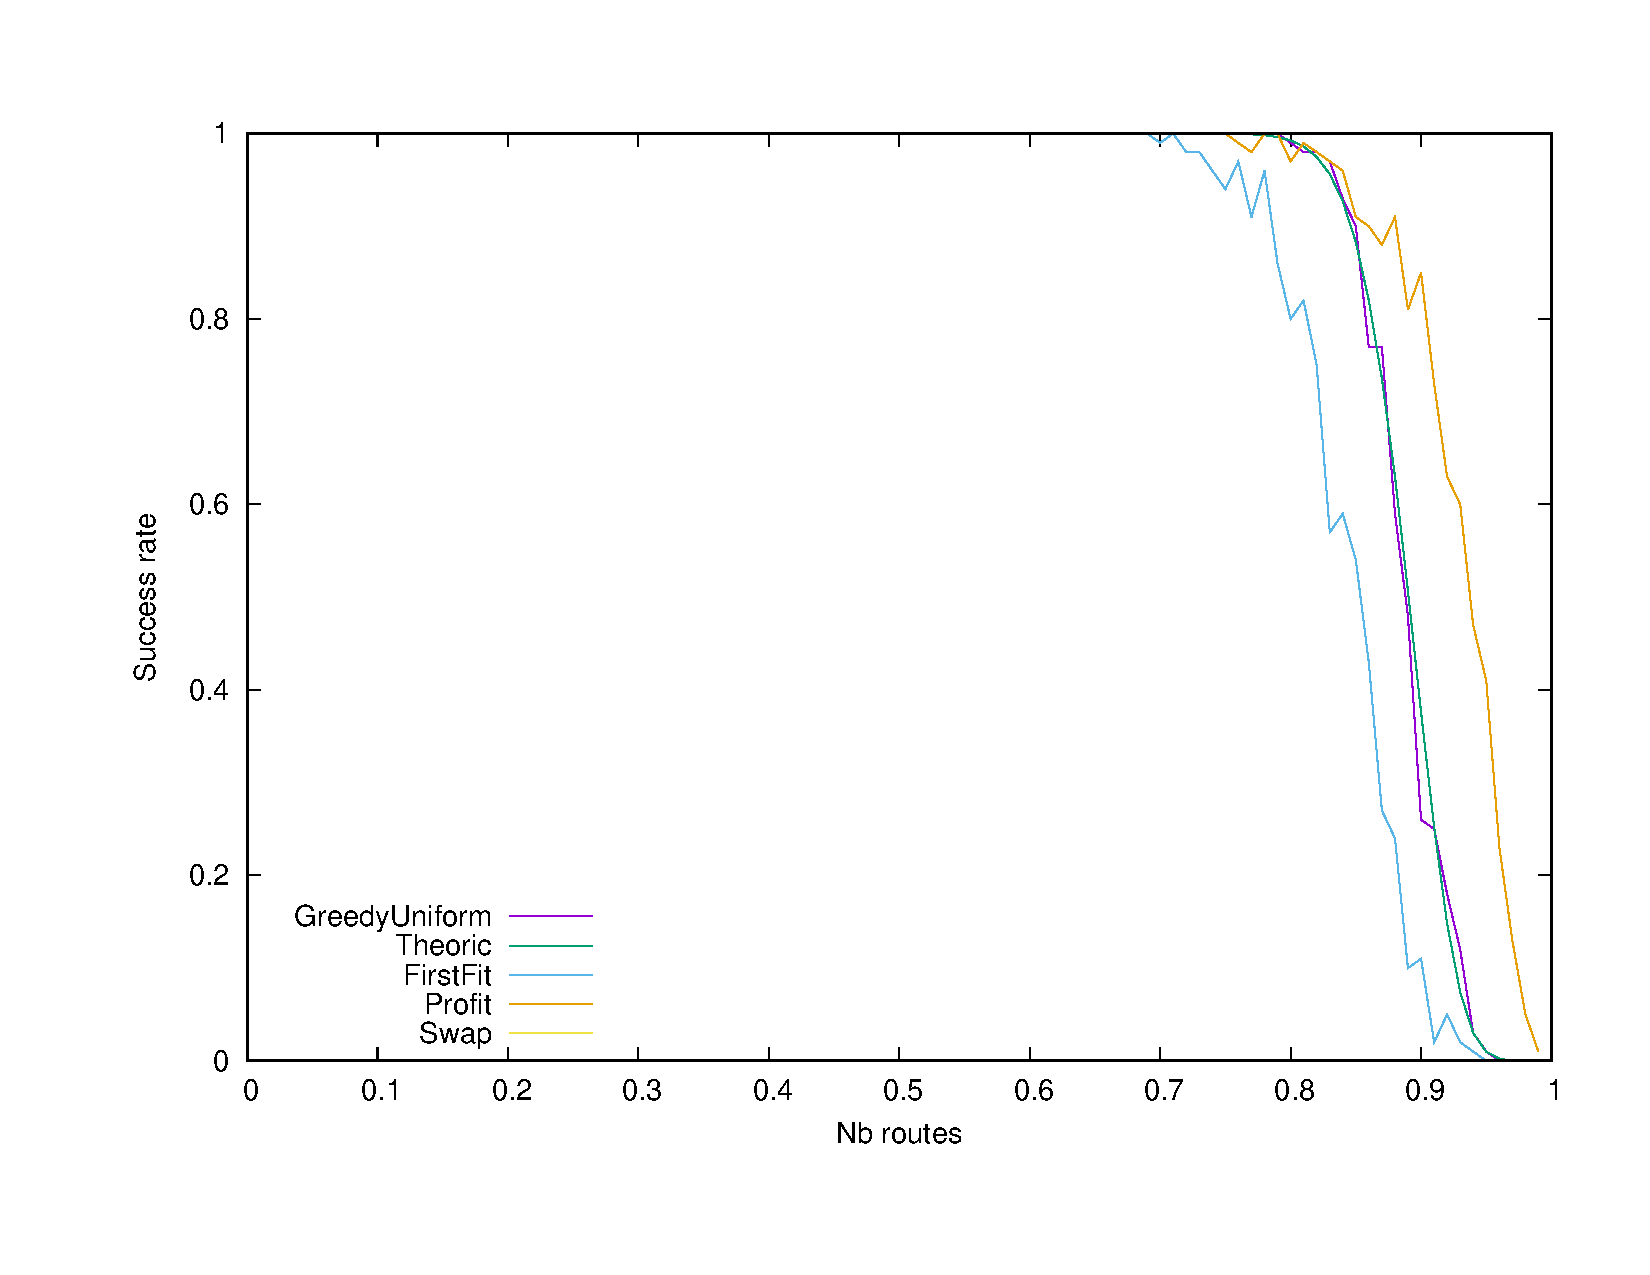
\includegraphics[scale=0.3]{success_tau1}
\end{center}
\caption{Success rate for $\tau = 1$ and $P=100$}
\label{fig:tau1}
\end{figure}

\begin{figure}
\begin{center}
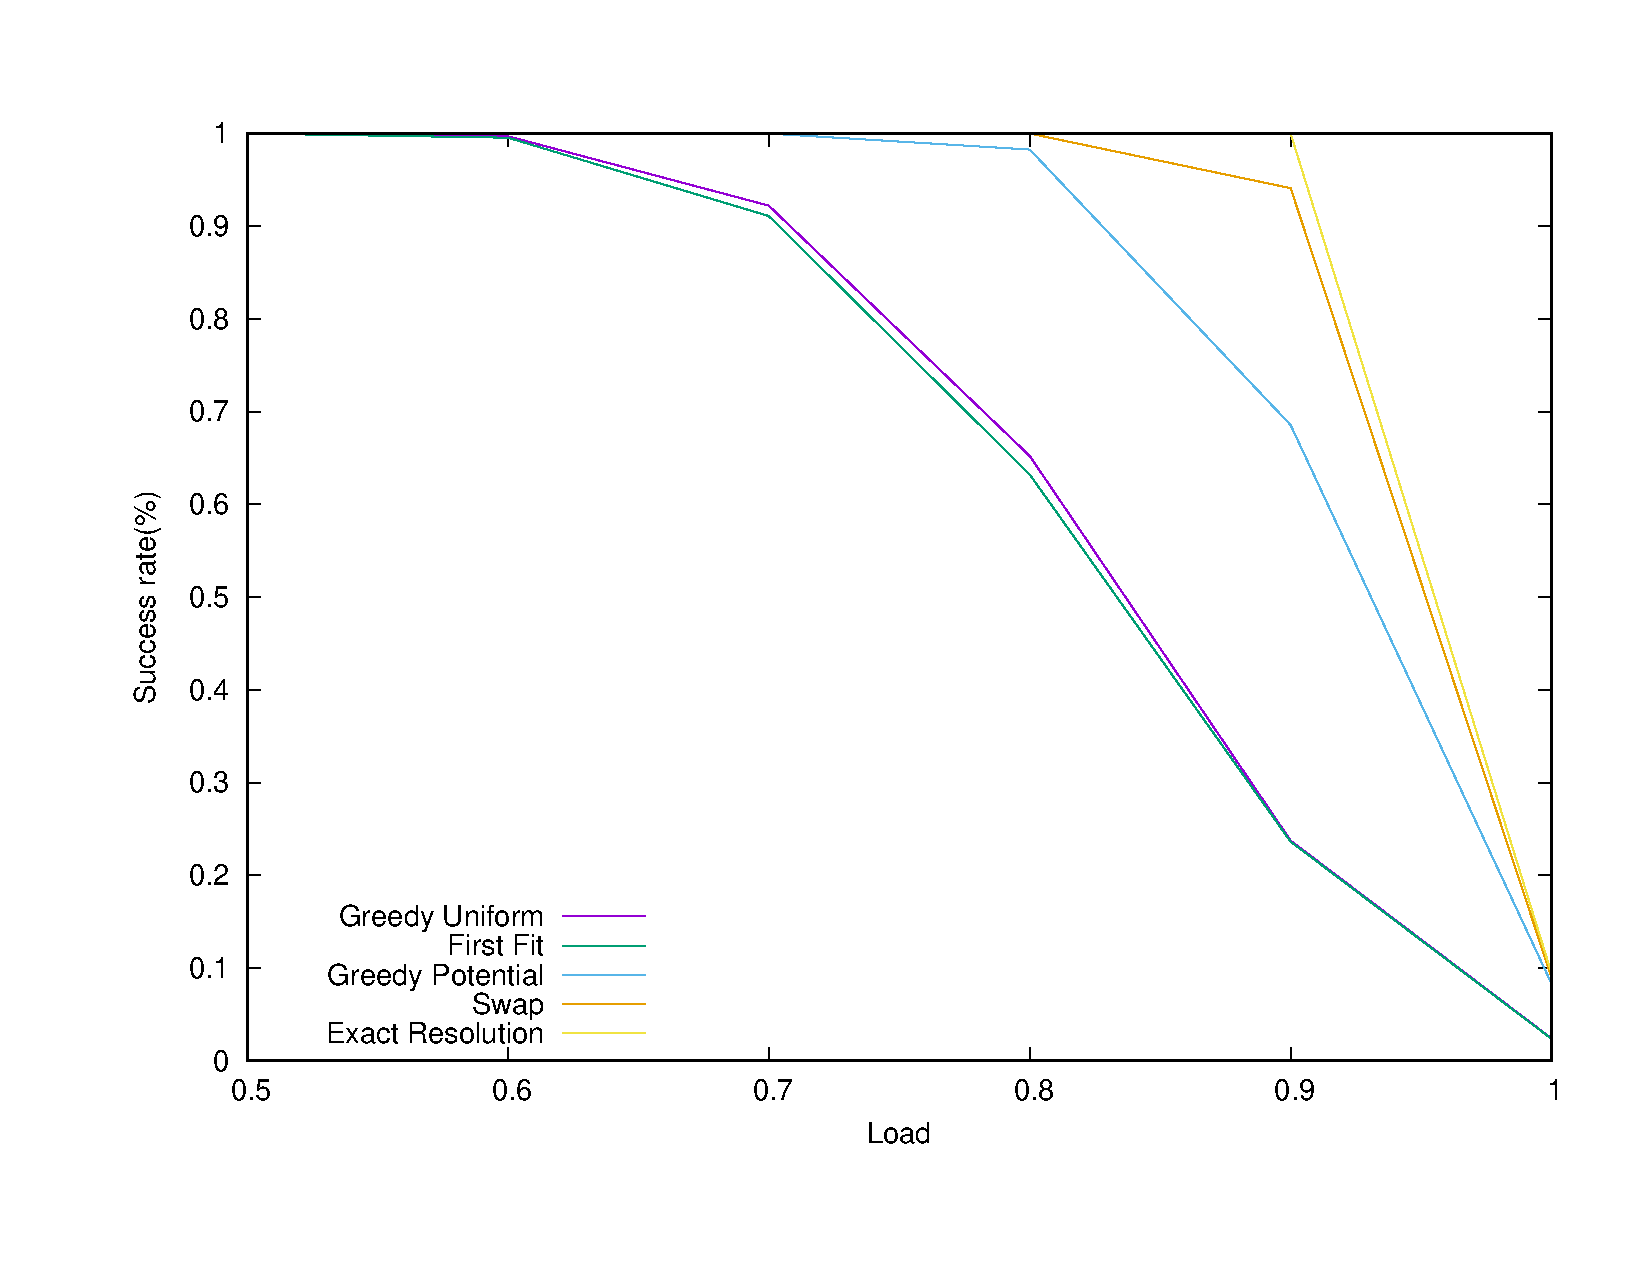
\includegraphics[scale=0.3]{tau110}
\end{center}
\caption{Success rate for $\tau = 1$ and $P=10$}
\label{fig:tau1-10mess}
\end{figure}

\section{Conclusion}

In this article, we have proved that there is always a solution to \pma and that it can be found in polynomial time 
for large $\tau$ and load  $0.4$ or for $\tau = 1$ and load $0.61$. Moreover, the performance of the presented algorithms over average instances are shown to be excellent empirically but also theoretically for Greedy Uniform.
Hence, we can use the simple algorithms presented here to schedule C-RAN messages \emph{without buffer nor additional latency}, if we are willing to use only half the bandwidth of the shared link. 

Many questions on \pma are still unresolved, the first one being its complexity.
Moreover, we plan to adapt the Swap algorithm to the case $\tau > 1$. While the potential
can be defined in the same way, it is not yet clear that it would help as much in this setting.
We could also analyze the behavior of the presented algorithms over random instances in the case $\tau > 1$.
For instance, it is possible to form very long compact tuples over random instances and we could
use that to obtain an algorithm which works with high probability for load less than $0.5$. 
First Fit or Meta Offset can easily be adapted to network topologies with more than a single link, but we could also try to adapt Compact Tuples and Swap. Finally, to capture networks carrying several types of messages, it would be interesting to allow for different message sizes, which makes methods using meta-offsets seemingly useless.



%\section{Lower bounds}

%Pour m=6, on peut toujours placer 5 éléments, que dire pour plus grand ?
%Remarque si tous les delais sont différents, on peut les placer, expliquer ça. 
%Example/family of examples for which some greedy alg fail -> facile pour le first fit
%Example/family of examples with a given load such that there are no feasible solution.

\bibliographystyle{ieeetr}
 \bibliography{Sources}

\end{document}
